\chapter{Implementation Details}
This chapter describes how the Phase~II system is built. Sections~5.1 and~5.2 record the development environment and the datasets. Section~5.3 describes the model and service implementation. Section~5.4 records how the metrics are kept reproducible. Section~5.5 presents the Phase~II application.

\section{Development Environment}
The project keeps the Phase~I repository shape. A pnpm workspace holds the TypeScript client with its shared engines. A uv workspace holds the Python packages, the service, and the research code. The two coexist so that the research code imports the same Python engines the service runs.

Table~\ref{tab:tools} lists the environment. The first eleven rows carry the Phase~I stack unchanged. The last seven rows add the Phase~II generation, grading, feedback, judgment, sandbox, embedding, and editor concerns.

\begin{table}[htbp]
\centering
\footnotesize
\caption{Development environment: tools and libraries. The first eleven rows carry the Phase~I stack; the last seven add the Phase~II loop.}
\label{tab:tools}
\begin{tabular}{p{4.0cm} p{8.4cm}}
\toprule
\textbf{Concern} & \textbf{Technology} \\
\midrule
Client language and build & TypeScript, Vite, pnpm workspace \\
Client UI & React~19 \\
Local-first storage & Dexie over IndexedDB \\
Intelligence service & Python~3.12, FastAPI, Uvicorn \\
Scientific stack & NumPy, SciPy \\
Service authentication & PyJWT, verifying Supabase-issued tokens \\
Containerisation & Docker Desktop on WSL2 (Compose) \\
Python workspace & uv \\
JavaScript testing & Vitest, fast-check (property tests), Playwright (end-to-end) \\
Python testing and linting & pytest, ruff \\
Backend and hosting & Supabase (auth, database, storage), Vercel \\
Generation provider & OpenRouter, \texttt{deepseek/deepseek-v4-flash-0731}, temperature 0.3, reasoning off, 30~s timeout \\
Rubric-grading model & \texttt{deepseek/deepseek-v4-flash-0731} through \texttt{GRADING\_MODEL}, the authoritative written-arm score \\
Feedback-copy model & \texttt{meta/muse-spark-1.3-contributor} through \texttt{FEEDBACK\_MODEL}, reasoning effort low \\
Judgment client & Jev-1.13 hosted System One API through \texttt{OPENROUTER\_JEV\_API\_KEY}, advisory shadow and loop-verdict judge \\
Code-execution sandbox & Piston sandbox profile on port~2000 for hidden-test grading \\
 GPU inference sidecar & Qwen3-Embedding-0.6B and Qwen3-Reranker-0.6B on port~8200 in a separate compose project \\
Client code editor & CodeMirror with an advisory Pyodide check that never grades \\
\bottomrule
\end{tabular}
\end{table}

\section{Datasets and Their Sources}
A single learner's real log does not supply a known ground truth for latent mastery and pace in this design. The Chapter~6 comparison therefore runs on fixed artifacts with planted and known properties. Table~\ref{tab:datasets} lists the datasets and the role each plays.

The frozen corpus is a single textbook (edition needs verification) at 754 chunks with 768-dimensional sidecar vectors. Three gold files score the offline leg against it: the objective probe set, the written gold set, and the coding gold set. The fixed folds and the attempt gate sit beside them in \texttt{eval\_golds.json}.

The longitudinal leg replays four synthetic archetypes with known posture: steady, crammer, struggling, and returning. Their generator plants weekly pace, skip behavior, gap weeks, and replan back-pointers explicitly. The Open University dataset (version needs verification) calibrates the Phase~I generator only and does not enter the Phase~II comparison. Real single-learner logs stay reserved for future validation and are not used here.

\begin{table}[htbp]
\centering
\footnotesize
\caption{Datasets used in Phase~II and their sources.}
\label{tab:datasets}
\begin{tabular}{p{3.6cm} p{3.8cm} p{5.0cm}}
\toprule
\textbf{Dataset} & \textbf{Source} & \textbf{Role} \\
\midrule
 Frozen corpus and harness golds & In-repository gold files: \texttt{eval\_golds.json} with probe, written, and coding sets. ACCA text at 754 chunks with 768-dimensional sidecar vectors (edition needs verification) & Primary ground truth for the offline leg: generation, retrieval, mastery, and coding checks \\
 Synthetic longitudinal histories & In-repository generator with four archetypes: steady, crammer, struggling, and returning & Whole-loop replay with known posture, and the post-fix replay evidence is versioned \\
 OULAD & Public Open University dataset (version needs verification) & Calibration source for the Phase~I generator \\
 Real session logs & The candidate's own sessions & Reserved for future validation, outside the Phase~II comparison \\
\bottomrule
\end{tabular}
\end{table}

\section{Model and Service Implementation}
Each algorithm has one behavioral definition. The client and service hold separate implementations only where the client must compute a view locally. The client-side engines are written in TypeScript, and a Python mirror of each engine runs behind the intelligence service. A golden-fixture parity harness keeps the two implementations aligned.

The TypeScript engines emit reference inputs and outputs. A Python test replays each input and asserts numeric equality within a 1e-6 relative and absolute tolerance. The shared numeric constants, such as the BKT parameters, stay identical on both sides.

The split between client and service follows the architecture of Figure~\ref{fig:architecture}. Service-side code owns grounded generation, per-family grading arms, and the mastery endpoint. It also owns the guide stream with its gated reveal. It further owns the feedback-copy endpoint and the loop verdict with the Jev judge as a hosted-API client. The client keeps the engines it must read locally. Those are the roadmap bookings, the Gaussian-process projection, the mastery readers with the difficulty chip, and the verdict handoff.

The offline research harness imports the production Python engines as candidates. It never re-implements them, so an offline result measures the same engine code the service runs. Listing~\ref{lst:bktforward} shows the shipped BKT forward filter, which realizes Equation~\ref{eq:bkt-update}, and Table~\ref{tab:packages} lists the main packages.

\noindent\begin{minipage}{\linewidth}
\begin{lstlisting}[language=Python, caption={The shipped BKT forward filter, which realizes Equation~\eqref{eq:bkt-update}.}, label={lst:bktforward}]
def bkt_forward(
    observations: list[MasteryObservation],
    params: BktParams = DEFAULT_PARAMS,
) -> tuple[list[float], list[float]]:
    """Run the forward filter over one skill's observation sequence.

    Returns ``(mastery_after, p_correct_before)`` parallel lists:
    ``p_correct_before[i]`` is the predicted probability of correctness for
    observation ``i`` computed from the belief before it, and
    ``mastery_after[i]`` is P(mastery) after processing observation ``i``.
    """

    mastery: list[float] = []
    p_correct: list[float] = []
    belief = params.p_init
    for obs in observations:
        p_correct.append((1.0 - params.p_slip) * belief + params.p_guess * (1.0 - belief))
        if obs.correct:
            numerator = (1.0 - params.p_slip) * belief
            denominator = numerator + params.p_guess * (1.0 - belief)
        else:
            numerator = params.p_slip * belief
            denominator = numerator + (1.0 - params.p_guess) * (1.0 - belief)
        belief = numerator / denominator if denominator > 0 else belief
        belief += (1.0 - belief) * params.p_learn
        mastery.append(float(np.clip(belief, 0.0, 1.0)))
    return mastery, p_correct
\end{lstlisting}
\end{minipage}

\begin{table}[H]
\centering
\footnotesize
\caption{Main packages and their roles.}
\label{tab:packages}
\begin{tabular}{p{4.8cm} p{7.6cm}}
\toprule
\textbf{Package / module} & \textbf{Role} \\
\midrule
\texttt{packages/progress} (TS) & Client mastery engine with bkt-v1: projection and the difficulty chip \\
 \texttt{packages/roadmap-engine} (TS) & Client booking and roadmap generation. The booking model is unchanged \\
\texttt{packages/py-progress} (Py) & Python mirror: Bayesian and enriched-shrinkage calibration, CUSUM, Gaussian process, bkt-v1 \\
\texttt{packages/py-roadmap-engine} (Py) & Python mirror of the roadmap engine \\
\texttt{services/intelligence} (Py) & FastAPI service with a portless worker: generation, grading, mastery, guide, feedback, and the loop verdict \\
\texttt{services/embedder} & Qwen3 embedding and rerank sidecar in a separate compose project \\
Piston sandbox & External image for hidden-test code execution, started on demand \\
 Research scripts & Offline harness and probes, importing the production engines \\
\bottomrule
\end{tabular}
\end{table}

Code answers execute in the self-hosted Piston sandbox through the profile on port~2000. Hidden tests and reference solutions stay server-side. The client runs visible tests only as advice. No resource or egress bound for that sandbox is stated in this report (see Section~6.6).

Table~\ref{tab:phase2-api} lists the Phase~II service surface. Every route verifies the signed Supabase token before any model runs. Every call sends one \texttt{X-Request-ID}, and failures answer with typed service errors that fail closed.

\begin{table}[htbp]
\centering
\footnotesize
\caption{Phase~II service surface: method, auth, contract, and errors.}
\label{tab:phase2-api}
\begin{tabular}{p{4.6cm} p{7.8cm}}
\toprule
\textbf{Route} & \textbf{Contract} \\
\midrule
\texttt{POST} \newline \texttt{/v1/assessments/generate} & One material, one family, one question. Tracked job. Rejects multi-family calls. Terminal states never retry \\
\texttt{POST} \newline \texttt{.../attempts} & One answer per question. Never touches hidden tests or reference solutions \\
\texttt{POST} \newline \texttt{/v1/guide/stream} & Server-sent events with monotonic sequence. Gated Reveal stays locked \\
\texttt{POST} \newline \texttt{/v1/guide/reveal} & Requires confirmation plus the owned attempt bound to the question \\
\texttt{GET} \newline \texttt{/v1/mastery}, \texttt{/recommendations} & Stateless per-skill estimate plus one-band advisory recommendation \\
\texttt{POST} \newline \texttt{/v1/feedback/copy} & Drafts text for updated entries only. Static fallback. Never alters a grade \\
\texttt{POST} \newline \texttt{/v1/loop/decision} & Judge proposes, code router disposes at evidence 0.5 and confidence 0.7 \\
\texttt{POST} \newline \texttt{/v1/retrieval/search} & Owner-scoped chunks. Optional rerank flag with top-k reorder \\
\bottomrule
\end{tabular}
\end{table}

\section{Evaluation Metrics and Reproducibility}
The metrics used to score each loop stage are defined in Table~\ref{tab:phase2-metrics} of Chapter~4. This section records how the project keeps them reproducible.

Three facts carry the reproducibility claim. First, every gate fails closed by default. The evaluation harness stays inert unless the caller passes \texttt{-{}-activate}. The loop router maps a judge failure onto \texttt{hold} through a typed service error. The grading arms return a deterministic fail-closed outcome for unusable input and never fabricate a score.

Second, every call carries one request identifier from the browser to the service logs. The client sends \texttt{X-Request-ID} on each intelligence call. The service echoes it on each response, and every error log line carries it. One identifier therefore joins the frontend, the backend, and the end-to-end evidence.

Third, a reader can re-run both legs from versioned inputs and the documented services. The offline leg needs \texttt{eval\_golds.json} with \texttt{eval\_harness.py} and the documented Supabase, sidecar, and judge access. The longitudinal leg needs the synthetic generator with the four archetypes and the versioned post-fix replay evidence.

Table~\ref{tab:phase2-hyperparams} records the hyperparameters a rerun must hold fixed. Table~\ref{tab:phase2-testing} records the test inventory behind the delivered code. There is no continuous-integration gate: verification is agent-run per the repository workflow, and coverage is not measured.

\begin{table}[htbp]
\centering
\footnotesize
\caption{Hyperparameters a rerun must hold fixed.}
\label{tab:phase2-hyperparams}
\begin{tabular}{p{4.8cm} p{7.6cm}}
\toprule
\textbf{Parameter} & \textbf{Value} \\
\midrule
Chunking & About 400 tokens per chunk with about 30 tokens of overlap \\
Embedding & 768 dimensions from the Qwen3 sidecar \\
Generation retrieval & Top 5 owner-scoped chunks per call \\
Endpoint search & Top 50 candidates before rerank \\
Generation model & Temperature 0.3, reasoning off, 30~s timeout, 4096 max output tokens \\
Repair & At most one repair. Hard format and citation gates \\
Attempt gate & K=5 over 3 fold hashes \\
BKT shipped params & $p_{\text{init}}$ 0.15, $p_{\text{learn}}$ 0.1, $p_{\text{slip}}$ 0.05, $p_{\text{guess}}$ 0.2 \\
Loop gates & Evidence 0.5, confidence 0.7 (\texttt{LOOP\_APPROVE\_AT}) \\
\bottomrule
\end{tabular}
\end{table}

\begin{table}[htbp]
\centering
\footnotesize
\caption{Test inventory behind the delivered code (counts collected 2026-10-23).}
\label{tab:phase2-testing}
\begin{tabular}{p{4.8cm} p{7.6cm}}
\toprule
\textbf{Suite} & \textbf{Inventory} \\
\midrule
Intelligence service & 976 pytest tests collected across 57 test files \\
App and engines & 65 vitest test files (unit plus provider tests) \\
Loop hook and feedback units & 37 hook tests and 77 feedback tests passing in the repo suite \\
Browser end to end & 33 Playwright spec files against the managed stack \\
Harness and probes & 11 unit tests on the harness pure functions \\
\bottomrule
\end{tabular}
\end{table}

\section{The Phase~II Application}
The working application realizes the selected models. This section presents the Phase~II additions. The Phase~I screens are unchanged. Phase~I delivered the planner with its session runtime, progress views, and roadmap lifecycle, and that substrate is unchanged.

This section follows five user-facing additions in order. Materials and ingestion (Section~5.5.1) is Phase~I substrate. Assessment generation (FR-9) and taking and review (FR-10) come next. Practice and guidance (FR-11, FR-12, FR-14) and feedback with the loop verdict (FR-13, FR-15) are the remaining Phase~II additions. The requirements behind them sit in Sections~3.3 and~3.4. Each subsection adds one stage to the flow diagram.

\subsection{Materials and Ingestion}
A material enters through the create page. The source grid offers plain text, PDF document, and web article side by side. The pipeline turns the upload into embedded chunks. The library card shows the material's current state until it is ready. A ready card offers practice instead of a status badge. A failed card keeps its badge with a retry action.

The detail page owns the rest of the lifecycle. It shows provenance and the outline, and it links onward to assessment and practice. Materials reach readiness in the library. Later subsections add the remaining stages to the chain in Figure~\ref{fig:appflow5}.

\begin{figure}[htbp]
\centering
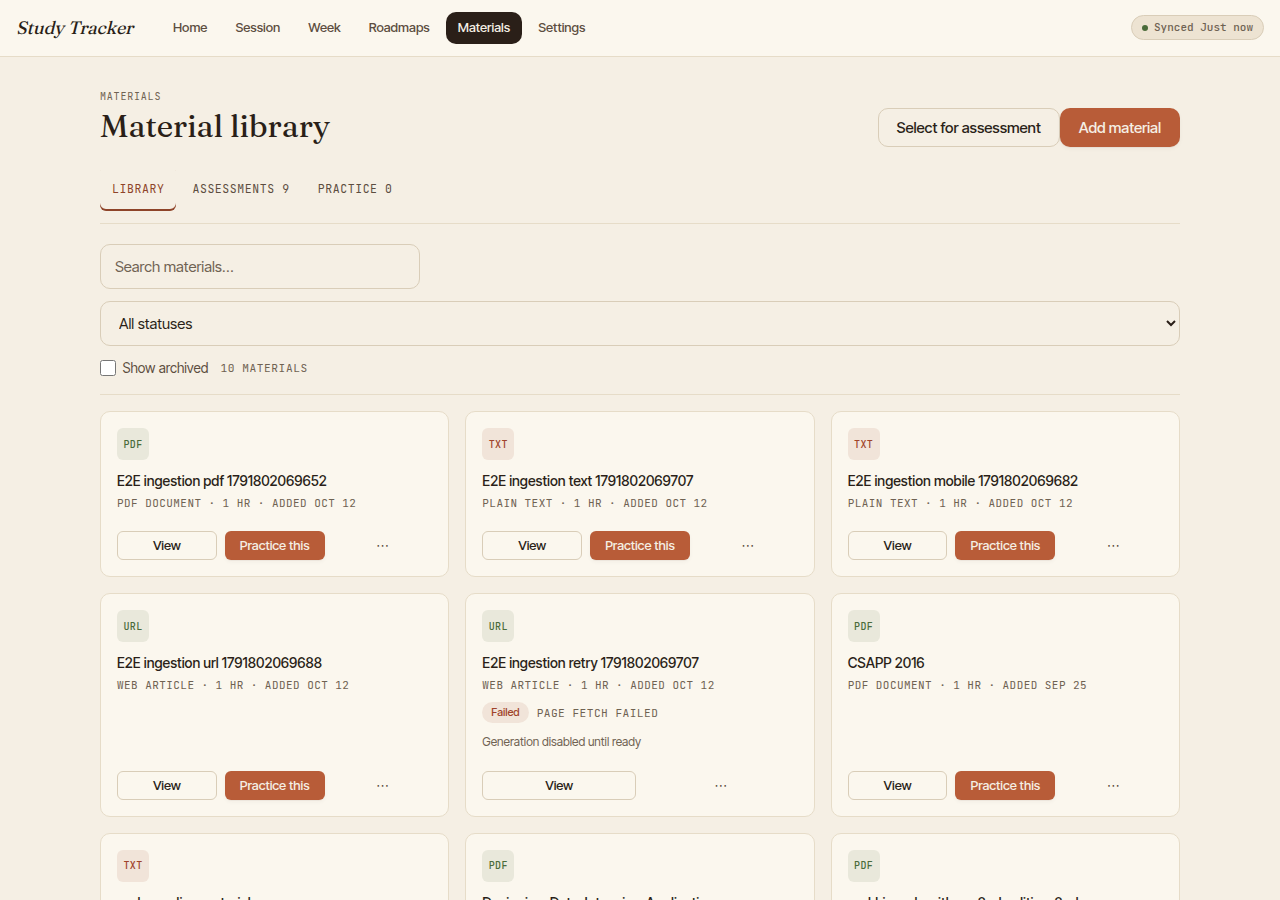
\includegraphics[width=0.85\linewidth, height=0.42\textheight, keepaspectratio]{screenshots/app_materials_library.png}
\caption{The material library: ready cards offer practice while the failed card keeps its badge with a retry action.}
\label{fig:appshot1}
\end{figure}

\subsection{Assessment Generation}
A generation run starts from the config page. The page binds one material, one family, and one scoped chapter before it requests a single question. The server gate admits exactly one family and one question per call. A mixed run alternates families across calls.

The assessment library lists every assessment with its family and status. Cache-first rows paint before revalidation completes. Generation runs as a tracked job. Only a run still marked generating retries in place. A failed run stays failed. Generation adds the second stage to the chain.

\begin{figure}[htbp]
\centering
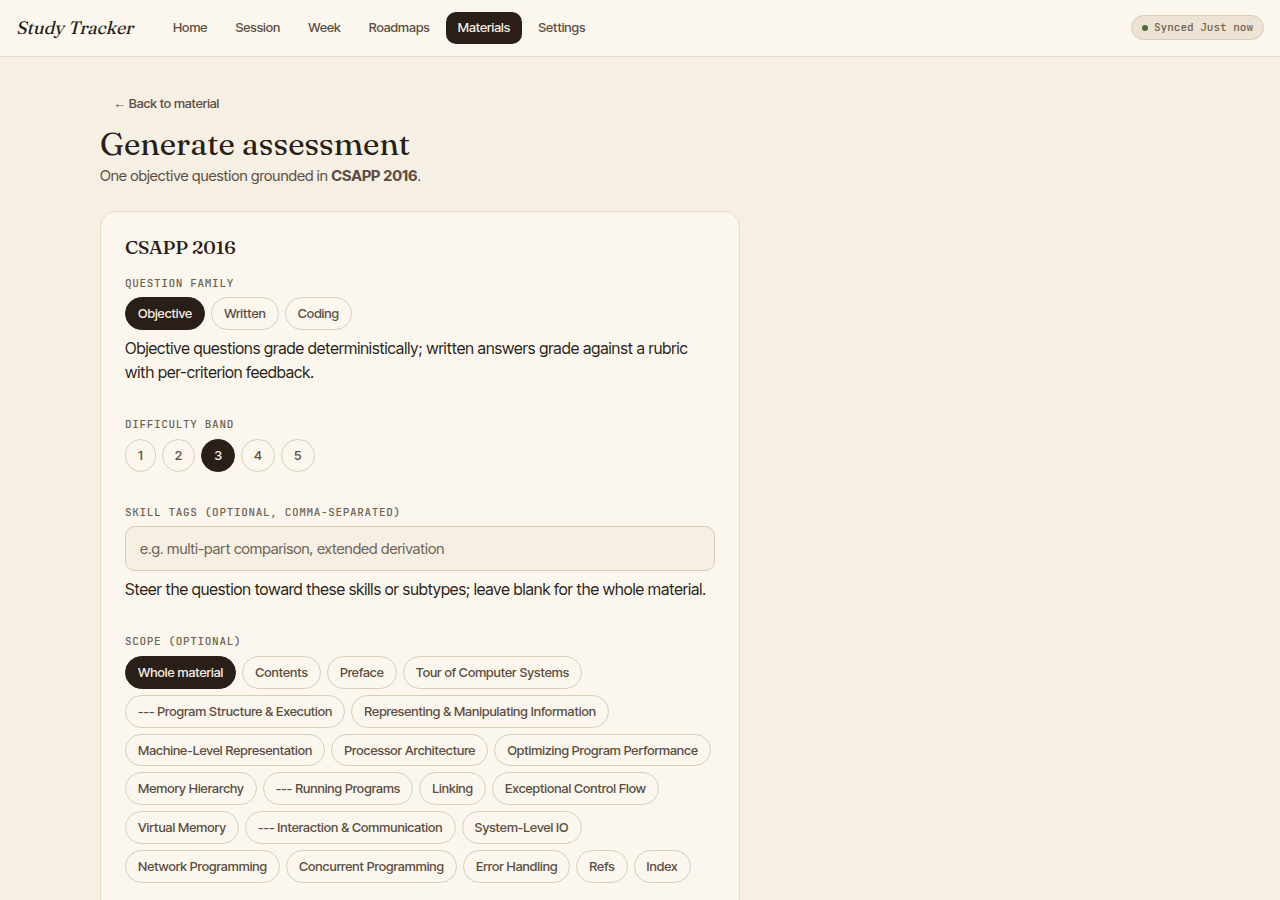
\includegraphics[width=0.85\linewidth, height=0.42\textheight, keepaspectratio]{screenshots/app_assessment_config.png}
\caption{Assessment generation: one material, one family, and one scoped chapter per question.}
\label{fig:appshot2}
\end{figure}

\subsection{Taking and Review}
The taking screens collect one answer per question. They never touch hidden tests, reference solutions, or authored accepted values. Objective answers compare exactly against values authored at generation time. Written answers go to the rubric arm, and coding answers execute against hidden tests. Coding runs in an embedded editor with an advisory client check. The server grade stays final, and no client result enters the record.

The review module shows each attempt beside its grade with per-question detail. Taking and review add the third stage to the chain.

\begin{figure}[htbp]
\centering
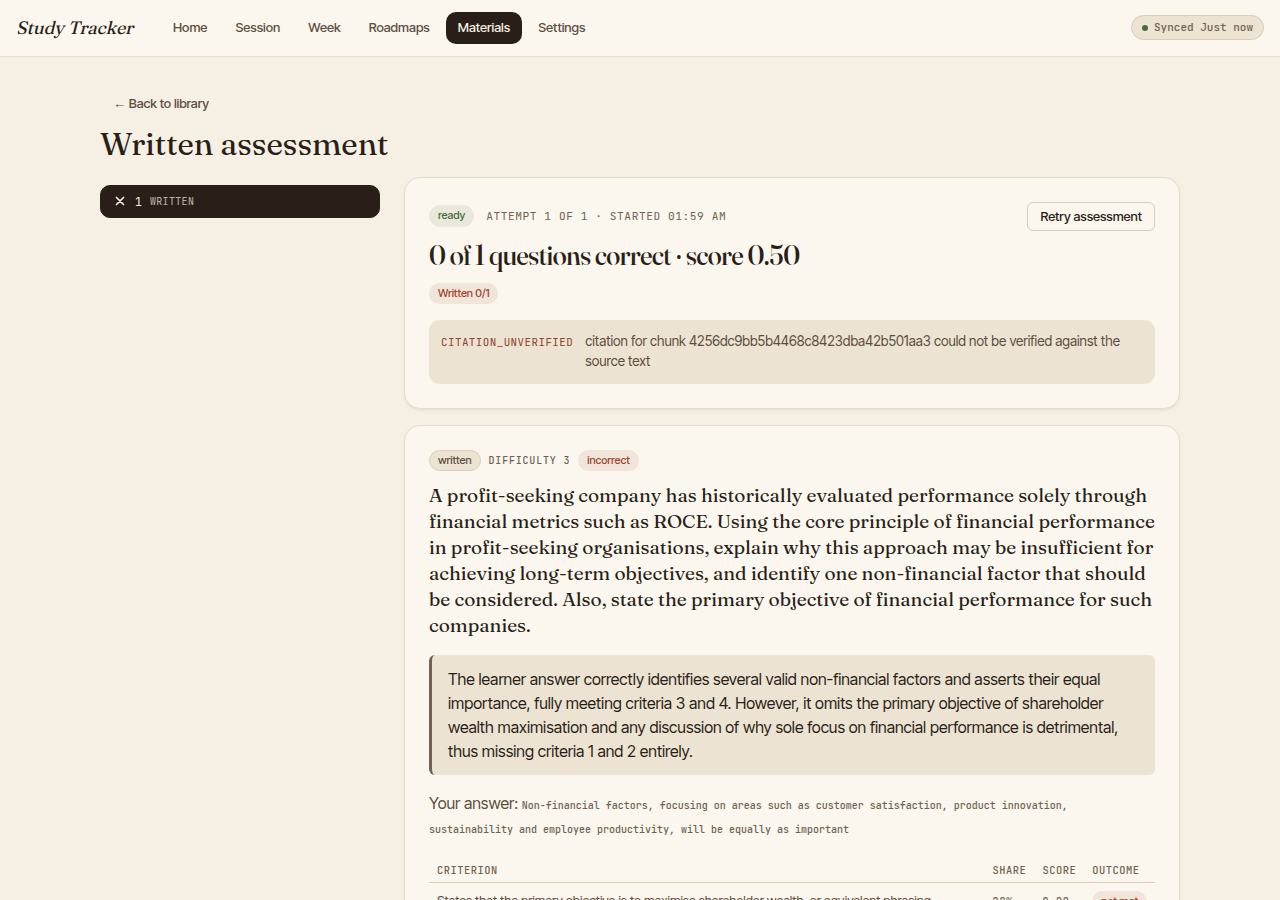
\includegraphics[width=0.85\linewidth, height=0.42\textheight, keepaspectratio]{screenshots/app_assessment_review.png}
\caption{Taking and review: the server grade with per-criterion rubric feedback.}
\label{fig:appshot3}
\end{figure}

\subsection{Practice and Guidance}
The practice hub gathers runs across materials. Each run resolves its questions lazily from the loaded assessments and stores no copies. Pause means leave and return. Neither finish nor abandon invents an observation.

The Socratic coach stays anchored to the page. It streams Nudge, Hint, and Targeted explanation against retrieved chunks and locks Reveal behind an explicit confirmation. The mastery reader beside it shows the current mastery estimate and its advisory, uncalibrated difficulty recommendation (Section~6.1). Practice and guidance add the fourth stage to the chain.

\begin{figure}[htbp]
\centering
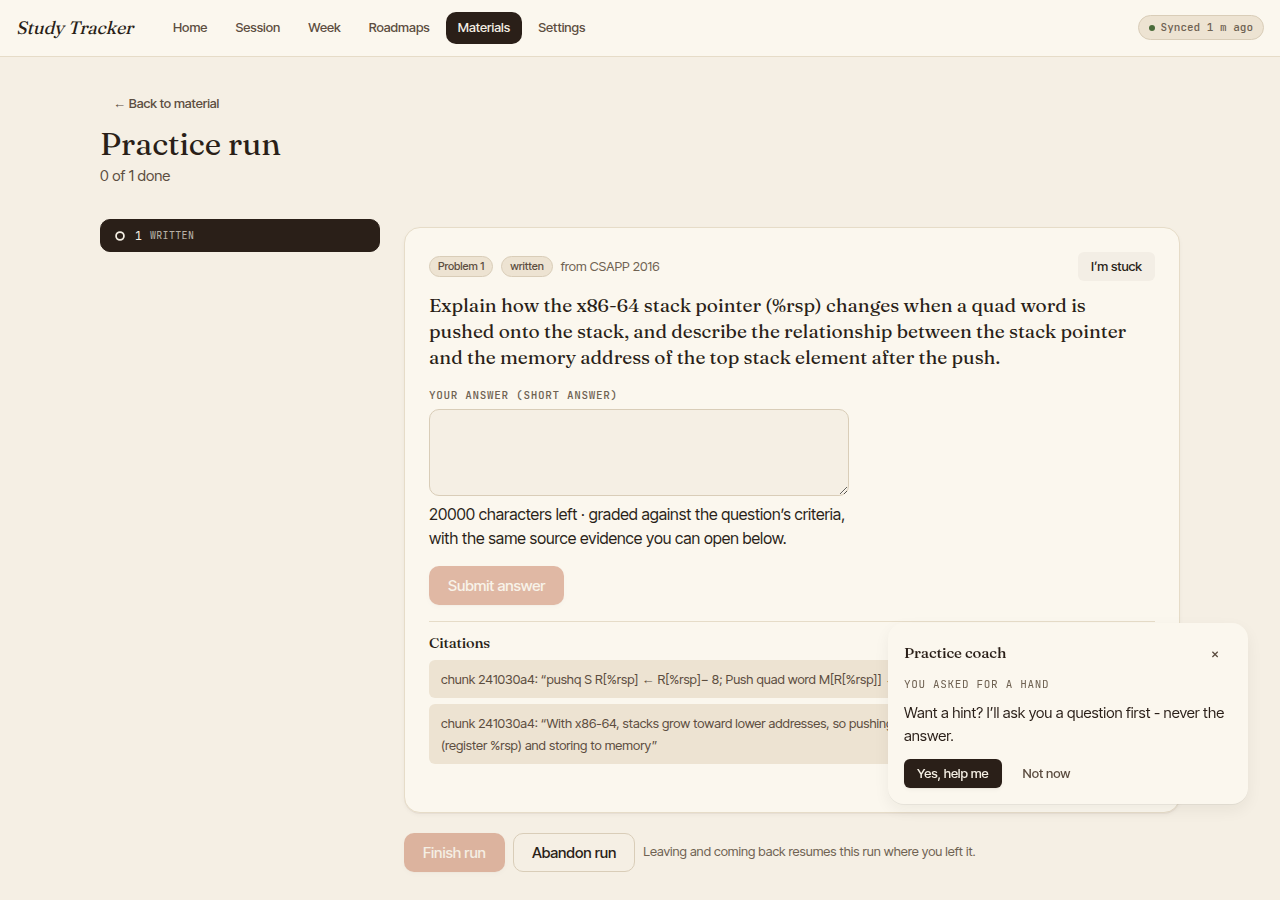
\includegraphics[width=0.85\linewidth, height=0.42\textheight, keepaspectratio]{screenshots/app_practice_run.png}
\caption{Practice run: the lazily resolved question with the Socratic coach anchored to the attempt.}
\label{fig:appshot4}
\end{figure}

\subsection{Feedback and the Closed Loop}
The roadmap detail page carries an evidence ledger. The ledger shows one of four states, cold, updated, stale, or rebuilding, derived from the cached mastery and the latest copy. The feedback-copy endpoint drafts text for updated entries only. The static fallback covers every other state, and the copy never alters a grade.

The loop verdict proposes one choice over the week. Only \texttt{suggest\_replan} passes its verdict pair to the replan screen. Confirming a replan mirrors the pair onto \texttt{RoadmapReplanned} and keeps the plan identity. \texttt{Keep} writes nothing. Figure~\ref{fig:appflow5} shows the complete chain.

\begin{figure}[htbp]
\centering
\begin{tikzpicture}[node distance=4mm and 8mm, font=\small, >=Latex,
  a/.style={draw, rounded corners=3pt, line width=0.8pt, align=center, inner sep=5pt, text width=2.1cm, fill=blue!4}]
\node[a] (M) {Materials\\\scriptsize (ingest, library)};
\node[a, right=of M] (G) {Generation\\\scriptsize (one family, one call)};
\node[a, right=of G] (T) {Taking, review\\\scriptsize (server grading)};
\node[a, right=of T] (P) {Practice, guide\\\scriptsize (runs, coach)};
\node[a, right=of P] (F) {Feedback, loop\\\scriptsize (verdict, replan)};
\draw[->] (M) -- (G); \draw[->] (G) -- (T); \draw[->] (T) -- (P); \draw[->] (P) -- (F);
\end{tikzpicture}
\caption{The complete Phase~II application flow: materials reach readiness, generation binds one family per question, taking collects answers under server grading, practice resolves lazily with the coach, and the verdict completes the chain.}
\label{fig:appflow5}
\end{figure}

\begin{figure}[htbp]
\centering
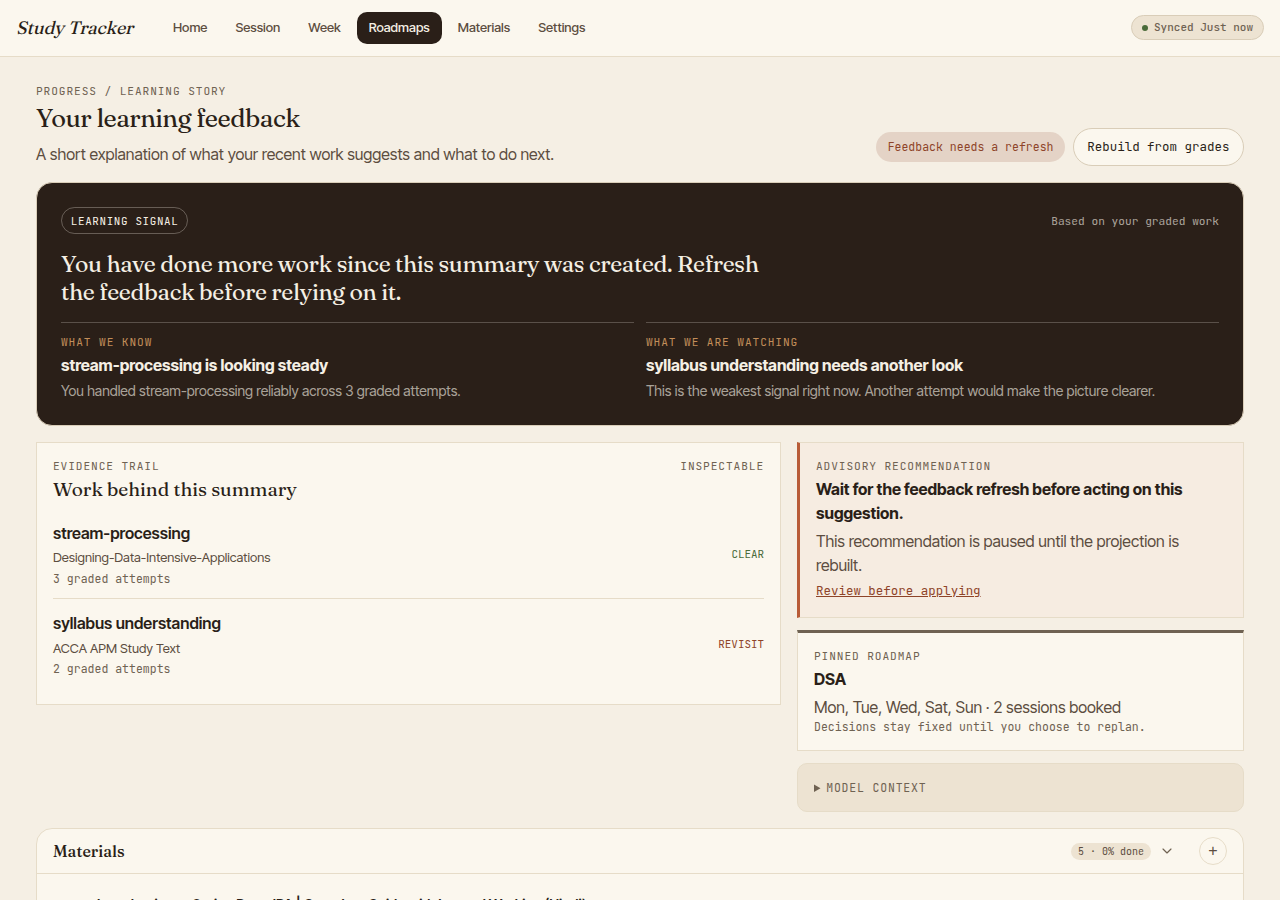
\includegraphics[width=0.85\linewidth, height=0.42\textheight, keepaspectratio]{screenshots/app_roadmap_evidence.png}
\caption{Feedback and the loop: the inspectable evidence trail with the advisory recommendation.}
\label{fig:appshot5}
\end{figure}

These five additions complete the Phase~II application. They are materials and ingestion, assessment generation, taking and review, practice and guidance, and the loop verdict with its replan. Chapter~6 reports the comparison behind them.
